\chapter{Verlinkung von Übungen}\label{linkUebung}
\begin{figure}[h!]
	\centering
	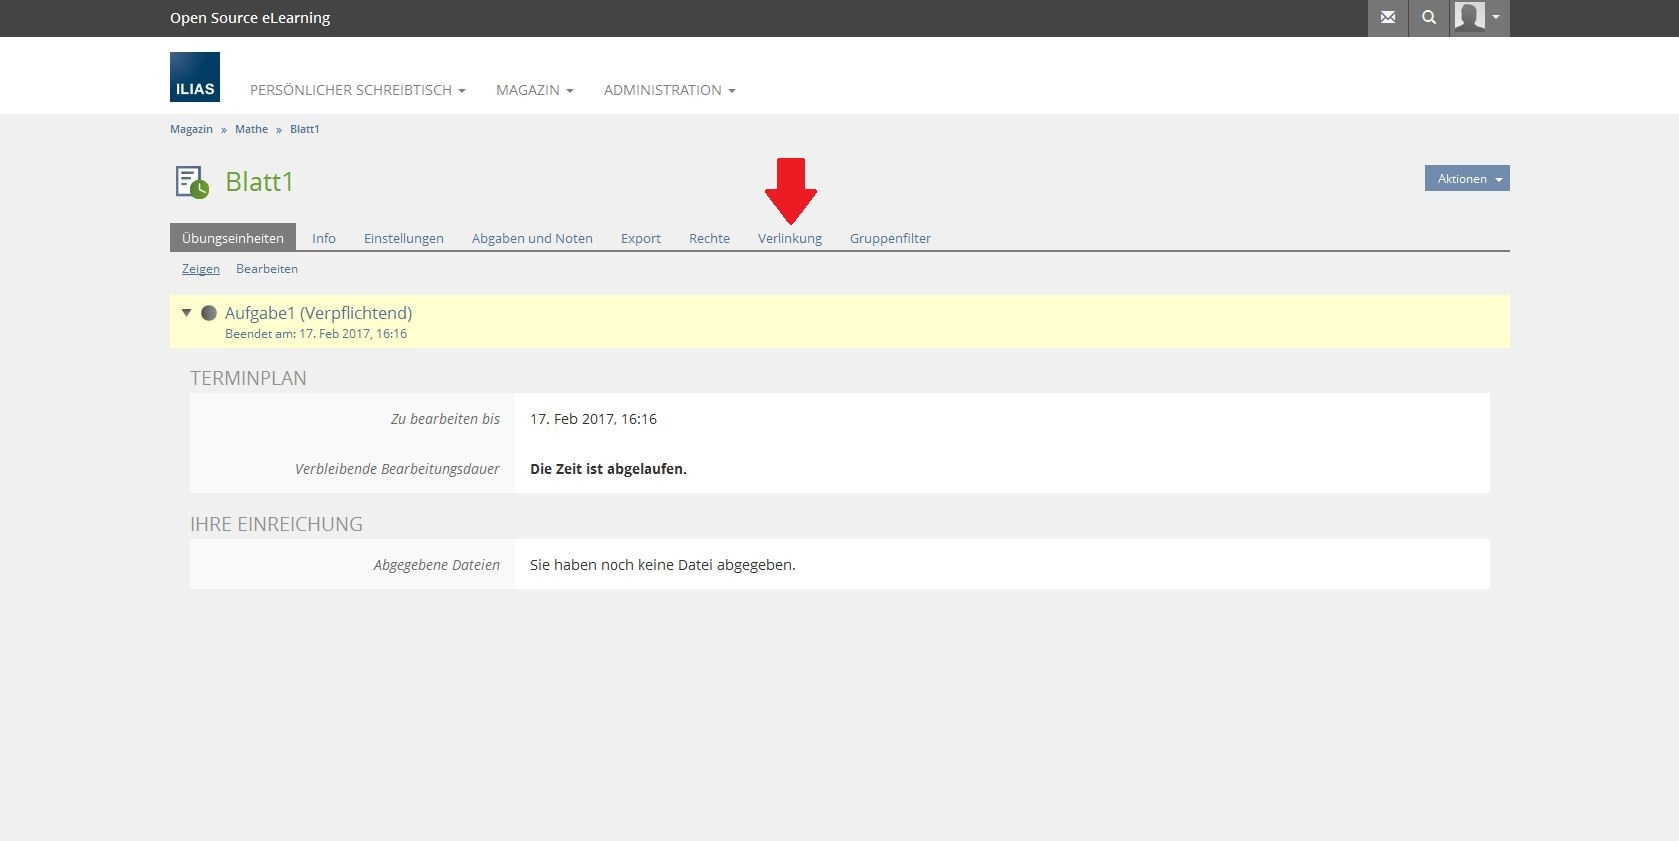
\includegraphics[width=1\textwidth]{img/excercise.jpg}
	\caption{Ansicht Verlinkung in Excercise/Übung}
\end{figure}

Bisschen Text 
\newpage

\section{Verlinkung von Übungen}
\begin{figure}[h!]
	\centering
	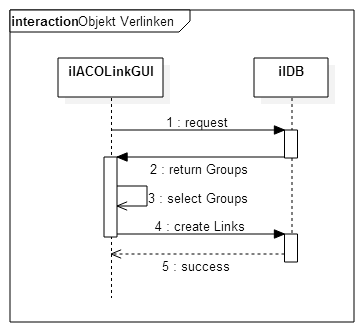
\includegraphics[width=.7\textwidth]{img/seq_linkGUI.png}
	\caption{Sequenzdiagramm Übung verlinken}
\end{figure}

\begin{figure}[h!]
	\centering
	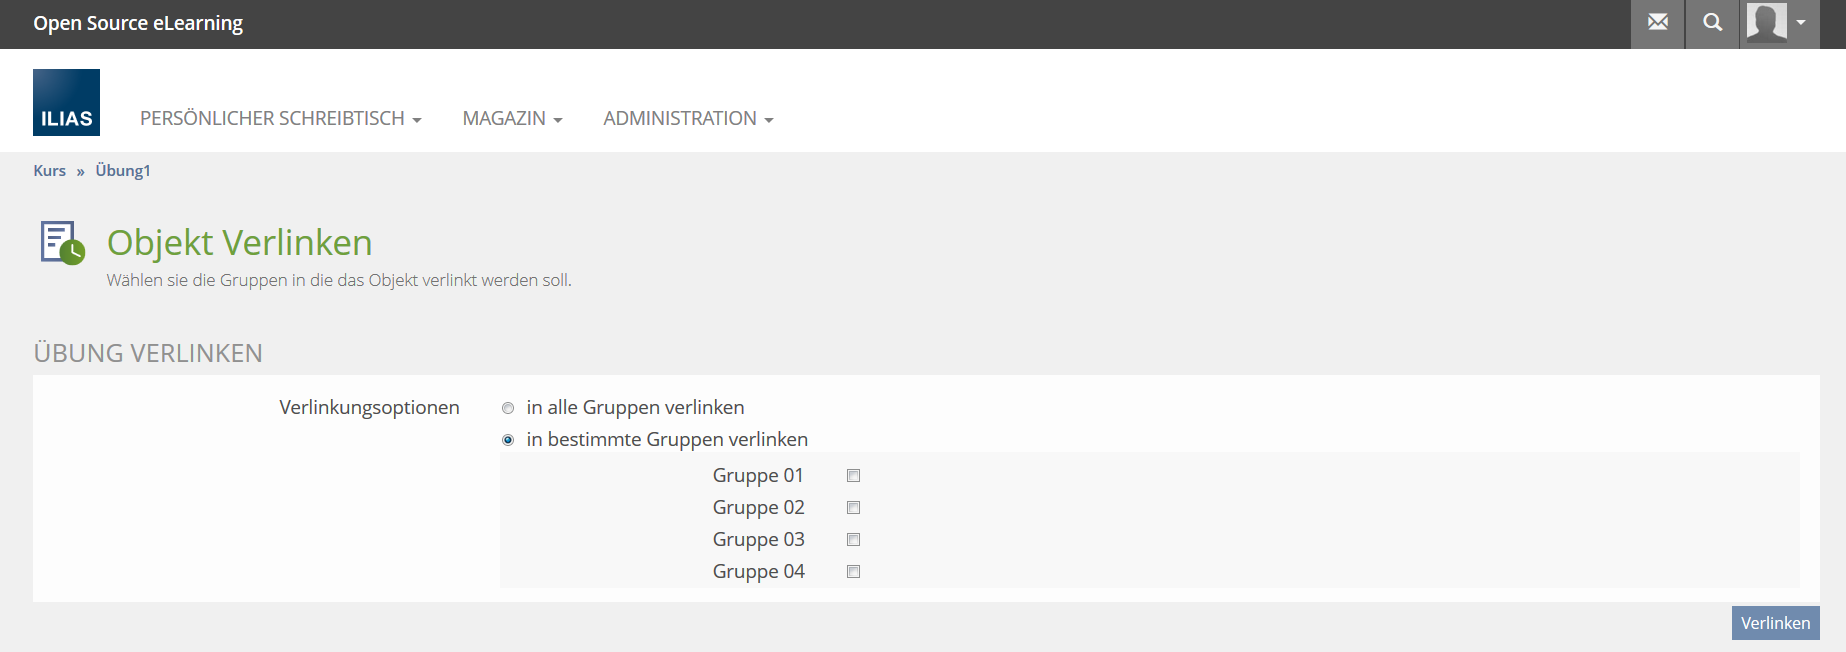
\includegraphics[width=1\textwidth]{img/linkUebung.png}
	\caption{Ansicht Link Übung}
\end{figure}

~\\Über eine Übung gelangen wir über den Tab Verlinkung zu dem dargestellten Bild. 
Mit der Funktion lässt sich diese Übung in die Gruppen des Kurses in dem die Übung existiert verlinken/verknüpfen. 
\newpage
\subsection*{in alle Gruppen verlinken}
\begin{itemize}
	\item Sollte dieser Radio Button ausgewählt und auf verlinken geklickt werden, so wird diese Übung in alle im Kurs vorhandenen Gruppen verlinkt. 
\end{itemize}

\subsection*{in bestimmte Gruppen verlinken}
\begin{itemize}
	\item Sollte dieser Radio Button ausgewählt werden erscheint eine Auswahl aller im Kurs vorhandenen Gruppen mit einer Checkbox
	\item Man kann jetzt einzelne Gruppen via der Checkbox markieren
	\item Klickt man auf "Verlinken" werden diese Gruppen verlinkt
\end{itemize}

~\\(Achtung: Duplikate werden von diesem Tab ausgeschlossen bzw. es wird nicht doppelt verlinkt, sollte die Übung schon in diese Gruppe verlinkt worden sein) 
\clearpage